% \AtBeginSection[]{
%     \begin{frame}
%         \frametitle{}
%         \tableofcontents[currentsection]
%     \end{frame}
% }

%%%%%%%%%%%%%%%%%%%%%%%%%%%%%%%%%%%%

\addtocounter{framenumber}{-1}

\section{Introduction}
\begin{frame}{Introduction}{MAS Design context}

    \begin{figure}
        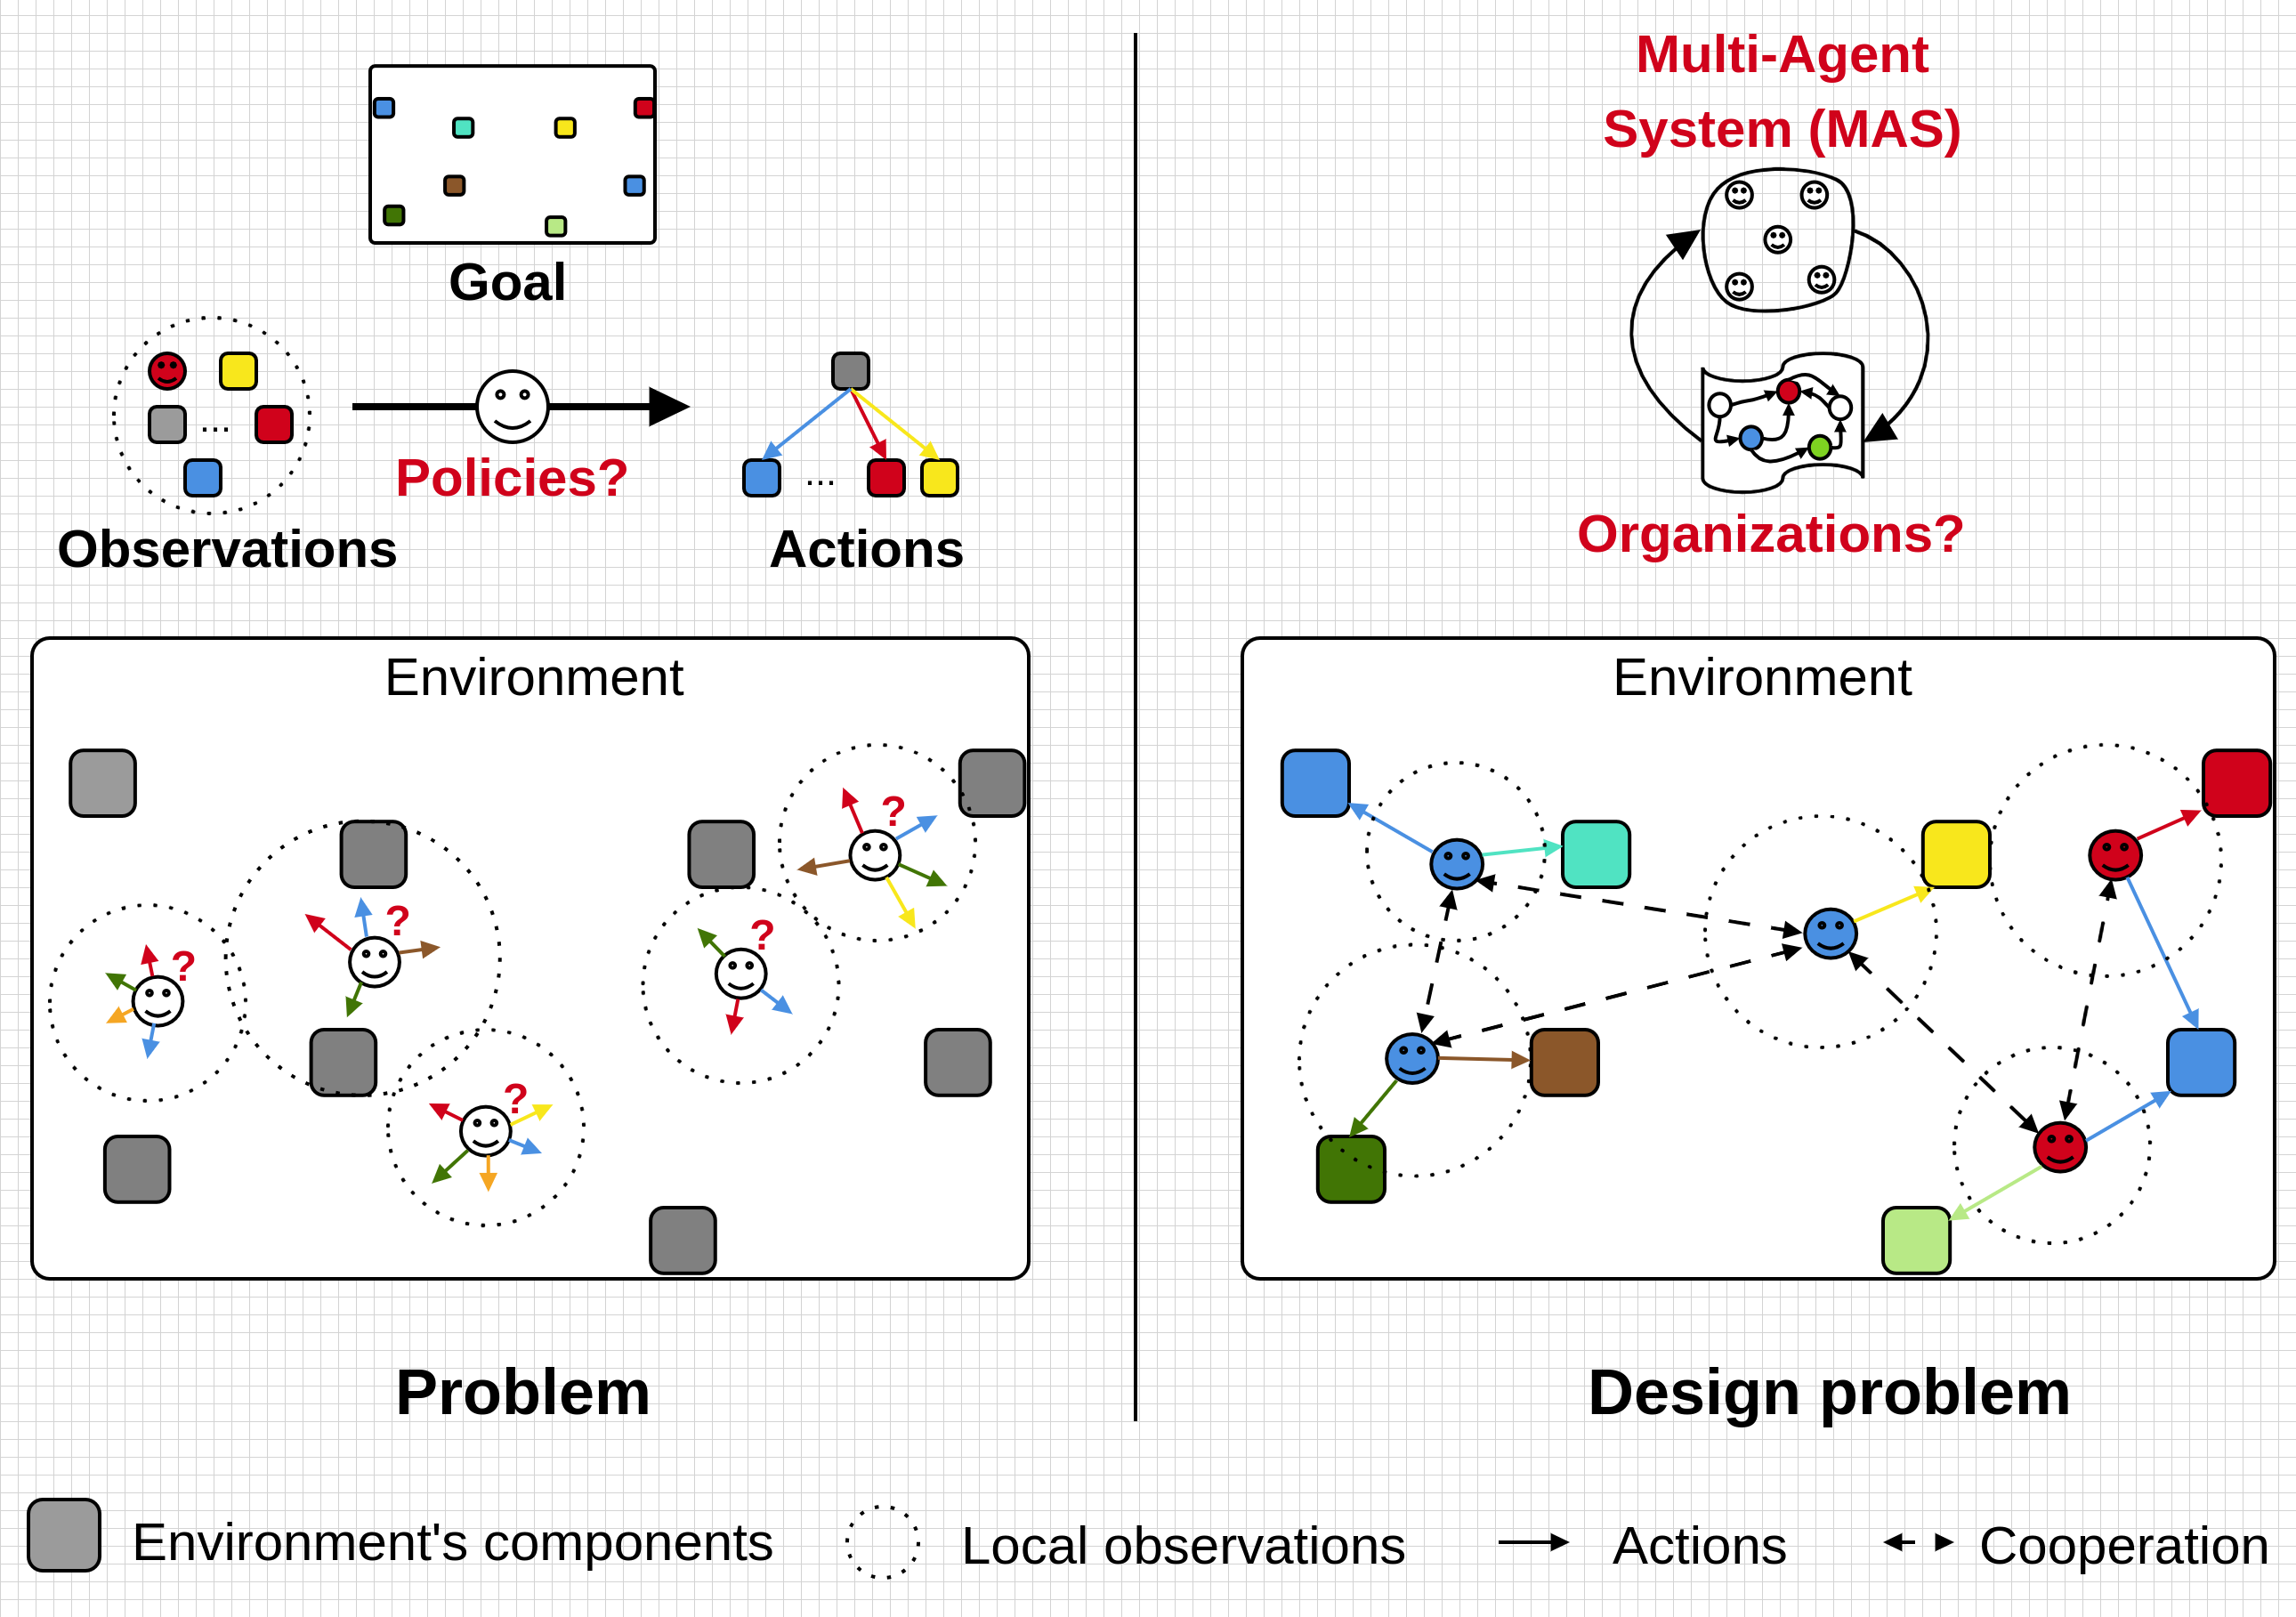
\includegraphics[width=0.7\linewidth]{figures/problem_illustration.png}
    \end{figure}

\end{frame}

\begin{frame}{Introduction}{Problem}


    \begin{alertblock}{Current design limitations}

        Methods require designers' experience but\dots
        \begin{itemize}
            \item \textbf{environment limitations}: complexity, limited access, non \dots
            \item \textbf{designers limitations}: availability, time consuming\dots
        \end{itemize}

        \vspace{-2ex}

        \begin{center}
            \begin{minipage}{11cm}
                \begin{block}{}
                    $\Longrightarrow$ \textbf{Problem}: Increasing design environment knowledge for design $\rightarrow$ \textbf{costly}
                \end{block}
            \end{minipage}
        \end{center}

        \vspace{-2ex}
        \begin{center}
            \begin{minipage}{0.95\linewidth}
                \centering
                \begin{exampleblock}{\textbf{Example}: Autonomous Intelligent Cyberdefense Agents~\cite{Kott2023} (AICA)}

                    \begin{columns}
                        \hspace{5ex}
                        \begin{column}{0.85\textwidth}
                            \textbf{Cyberdefense Multi-Agent System}: malware identification, countermeasures\dots \\
                            $\Longrightarrow$ No visual/intuitive comprehension of complex networked environments
                        \end{column}
                        \begin{column}{0.22\textwidth}
                            \hspace{-2.5ex}
                            
\includegraphics[width=0.8\linewidth]{figures/AICA_IWG.jpg}
                        \end{column}
                    \end{columns}

                \end{exampleblock}
            \end{minipage}
        \end{center}

    \end{alertblock}

    \begin{alertblock}{Targeted gaps}
        \begin{enumerate}
            \item[\phantom{X} (G1)] \textbf{Automating the search for suitable agents' policies satisfying design constraints};
            \item[\phantom{X} (G2)] \textbf{Explicating the emerging organizational mechanisms to assist the hand-craft design}.
        \end{enumerate}
    \end{alertblock}

\end{frame}
\begin{frame}{Introduction}{Addressing the gaps}

    \begin{alertblock}{Targeted gaps}
        \begin{enumerate}
            \item[\phantom{X} (G1)] \textbf{Automating the search for suitable agents' policies satisfying design constraints};
                \\ $\Longrightarrow$ Multi-Agent Reinforcement Learning (MARL)?
            \item[\phantom{X} (G2)] \textbf{Explicating the emerging organizational mechanisms to assist the hand-craft design}.
                \\ $\Longrightarrow$ Organizational Model (OM)?
        \end{enumerate}
    \end{alertblock}


    \begin{table}[]

        \centering
        \begin{tabular}{@{}ccc
                >{\columncolor[HTML]{FFFFFF}}c clc@{}}
            \toprule
            \cellcolor[HTML]{FFFFFF}{\color[HTML]{FFFFFF} }                                                                                                                                  &
            \textbf{MARL}                                                                                                                                                                    &
            \textbf{OM}                                                                                                                                                                      &
            \cellcolor[HTML]{FFFFFF}{\color[HTML]{000000} }                                                                                                                                  &
            \textbf{OM + MARL = OMARL}                                                                                                                                                       &
                                                                                                                                                                                             &
            \\ \cmidrule(r){1-3} \cmidrule(lr){5-5}
            \textbf{(G1)}                                                                                                                                                                    &
            \cellcolor[HTML]{FFFFFF}{\color[HTML]{34FF34} \begin{tabular}[c]{@{}c@{}}\small Find suitable\\ \small policies automatically\end{tabular}}                                      &
            \cellcolor[HTML]{FFFFFF}{\color[HTML]{FE0000} \small No automated way}                                                                                                           &
            \cellcolor[HTML]{FFFFFF}{\color[HTML]{000000} }                                                                                                                                  &
            \cellcolor[HTML]{FFFFFF}{\color[HTML]{34FF34} \begin{tabular}[c]{@{}c@{}c@{}}\small Find suitable\\ \small policies automatically\\ \small \phantom{XXX}\end{tabular}}           &
                                                                                                                                                                                             &
            \\

            \textbf{(G2)}                                                                                                                                                                    &
            \cellcolor[HTML]{FFFFFF}{\color[HTML]{FE0000} \begin{tabular}[c]{@{}c@{}}\small No explicit cooperation\\ \small /organization scheme\end{tabular}}                              &
            \cellcolor[HTML]{FFFFFF}{\color[HTML]{34FF34} \begin{tabular}[c]{@{}c@{}}\small Formalize implicit\\ \small organization as\\ \small Organizational Specifications\end{tabular}} &
            \multirow{-3}{*}{\cellcolor[HTML]{FFFFFF}{\color[HTML]{000000} \vspace{4ex}$\Longrightarrow$}}                                                                                   &
            \cellcolor[HTML]{FFFFFF}{\color[HTML]{34FF34} \begin{tabular}[c]{@{}c@{}}\small Formalize implicit\\ \small organization as\\ \small Organizational Specifications\end{tabular}} &
            \multirow{-3}{*}{\vspace{4ex}$\Longrightarrow$}                                                                                                                                  &
            \multirow{-5}{*}{\textbf{ \begin{tabular}[c]{@{}c@{}c@{}} \small Assisted \\ \small Design\\ \small Approach...\end{tabular}}}                                                     \\ \bottomrule
        \end{tabular}
    \end{table}

    % \begin{prosblock}{Contribution: AOMEA}

    %     \textbf{Assisted MAS Organization Engineering Approach (AOMEA)} based upon:
    %     \begin{itemize}
    %         \item \textbf{Multi-Agent Reinforcement Learning (MARL)}: automatically find suitable joint-policies;
    %         \item \textbf{Organizational model (OM)}: formalize an implicit organization as \textbf{Organizational Specifications (OS)};
    %         \item \textbf{Link MARL \& OM}: link explicit OS with \textbf{histories}/\textbf{trajectories} of on-training policies.
    %     \end{itemize}

    %     \

    %     In order to:
    %     \begin{enumerate}
    %         \item \textbf{Constrain MARL}: design constraints to satisfy during training to achieve the goals;
    %         \item \textbf{Generate Organizational specifications}: automatically compute OS from agents' behaviors.

    %               $\rightarrow$ exploitable insights into relevant mechanisms for MAS design.
    %     \end{enumerate}

    % \end{prosblock}


\end{frame}